In this section we describe two well-known anonymity protocols 
from the literature, and their variations, 
the leakage analyses of which we performed. 
%
%the \emph{Dining Cryptographers} \cite{dining} and \emph{Crowds} \cite{crowds}. 
%We implemented two variations of each in PRISM, and compared them with regard 
%to the QIF quantities introduced in Section~\ref{sec:prelqif}.

\subsection{The Dining Cryptographers protocol}

The \emph{Dining Cryptographers (DC)} anonymity protocol was proposed by 
David Chaum \cite{dining}. 
It is usually described within the following setting. 
Three cryptographers are invited by the NSA 
(The U.S. National Security Agency) to have dinner at a restaurant. 
Along with the invitation, one of them might have been secretly told by 
the NSA to pay the bill. 
Otherwise, the NSA itself would pay. 
The cryptographers wish to know whether one of them was asked to pay the bill
(as opposed to the NSA paying the bill), without revealing, however, which 
one of them is the payer. 
In order to do so, they execute the following protocol. 

Sitting in a round table, each cryptographer flips a coin, and shares the 
result with the cryptographer to their right. 
In this way each cryptographer sees the results of only two of the coins: the one he 
himself flipped, and the one flipped by the cryptographer sitting to his 
left. 
Each cryptographer then makes a public announcement. 
If he is not paying the bill, he announces 0 if the results of the two coins he
sees are the same (i.e., both heads or both tails), and announces 1 if they are 
different. 
However, if the cryptographer is the payer, he announces 1 if the results of the 
two coins coincide, and announces 0 otherwise.

The cryptographers now can learn whether the NSA is paying: 
if the sum of all three announcements (modulo 2) equals 0, 
the NSA is paying. 
If the sum equals 1, then one of them is paying. 
This can be easily seen from the fact that the announcement of 
each cryptographer not paying the bill is the number of heads he 
has seen (modulo 2). 
If no one is paying, then the final result is equal to twice the 
number of coins that landed heads up to modulo 2, which is certainly 0. 
If one of them is paying, however, the final result will be 1.

If the coins are fair, the identity of the cryptographer who pays the bill 
is totally preserved, both in relation to the other two cryptographers and to 
any external observer. 
If the coins are biased, however, the announcements made by the cryptographers 
might make one of them more likely to be the payer than the others. 
For example, if the coin tosses are very likely to yield tails, and only one 
cryptographer announces 1, then he is probably paying the bill.

We are specially interested in scenarios with a biased coin, for some 
information is leaked by the protocol.
We can use QIF to precisely quantify this leakage and we can determine 
by how much the attacker can improve his guessing strategy.
In this paper we study two different generalizations of the DC protocol, 
which expand the number of cryptographers involved.

\subsubsection{The cycle-DC variation.}

Our first variation of the DC protocol is akin to the original,
but the number of cryptographers can be any integer greater than 2.
Similarly to the original protocol, the cryptographers are arranged in 
a circular table, each tosses a coin and shares the result to the 
cryptographer at his right. 
\commentM{\qm{to} his right?}
The announcements are made in the same manner as before.
Also in this scenario, one of the cryptographers is the payer 
if, and only if, the sum of the announcements (modulo 2) equals 1. 

\subsubsection{The complete-DC variation.}

In our second variation of the DC protocol, all pairs of cryptographers 
share a coin toss result (i.e., they form a clique). 
If there are $N$ cryptographers, each one has access to $N{-}1$ coin-toss results.
After all the coin tosses are made, each cryptographer computes the number 
of heads he has seen (modulo 2). 
If he is not paying for the bill, this is the number that he announces. 
If he is paying, however, he inverts the announcement. 
Since each heads is counted twice, we also have that one of the 
cryptographers is paying if, and only if, the sum of the announcements (modulo 2) 
equals 1. 

\subsection{The Crowds protocol}

The \emph{Crowds} protocol was first devised to protect anonymity on web transactions. 
Suppose there is a group of users who wish to make requests to a server, 
without revealing their identities to that server. 

The users agree to cooperate on the protocol, and take the following steps.
(1) If a user wants to send a request (we call such user an \emph{initiator}), 
he chooses at random a user in the group (including himself), and forwards the 
request to this user.
(2) If a user receives a request, he forwards it to a random user with 
probability $p_f$, and forwards it directly to the server with probability $1{-}p_f$.
The second step is repeated until the request reaches the server. 

The protocol protects the initiator's identity because, after being 
forwarded for the first time, the request has an equal probability of 
landing at any user of the system. 
Therefore, the server does not acquire any information by observing 
which user sent the request to him at the end of the process.

The analysis of the protocol becomes more interesting when there are 
some \emph{corrupt} users in the group. 
These corrupt users are in collusion with the server, and reveal to 
it the identity of any regular user that sent them a request---in this case, 
we say that the regular user in question was \emph{detected}. 
Because the initiator must be in any path of the message on its way to the server, 
whenever a user is detected, he is the most likely to be the initiator. 
As expected, the level of anonymity provided by the protocol in this scenario depends 
on the number of users, on the number of corrupt users, and on the probability $p_f$.

In this paper we consider two variants of the Crowds protocol.

\subsubsection{The (original) Crowds variation.} 

In this variation, each user can communicate with any
other user (they form a clique), and there is \review{no} restriction 
on who can forward a message to whom.

\subsubsection{The grid-Crowds variation.} 
A common variation of this protocol \review{occurs} when a user 
is able to forward a request only to a subset of the remaining users. 
One particular instance of this scenario is when users are placed on 
a grid, as illustrated in Figure~\ref{figure:crowdsgrid}.
Edges represent users who can communicate, and we consider the edges going 
off the grid to connect users at opposite sides, e.g.,
user 1 is connected to users \review{2, 3, 4 and 7}. 
We consider that every user can \review{also} communicate directly \review{with} the server.

\begin{wrapfigure}{r}{0.25\linewidth}
\vspace{-10mm}
\centering
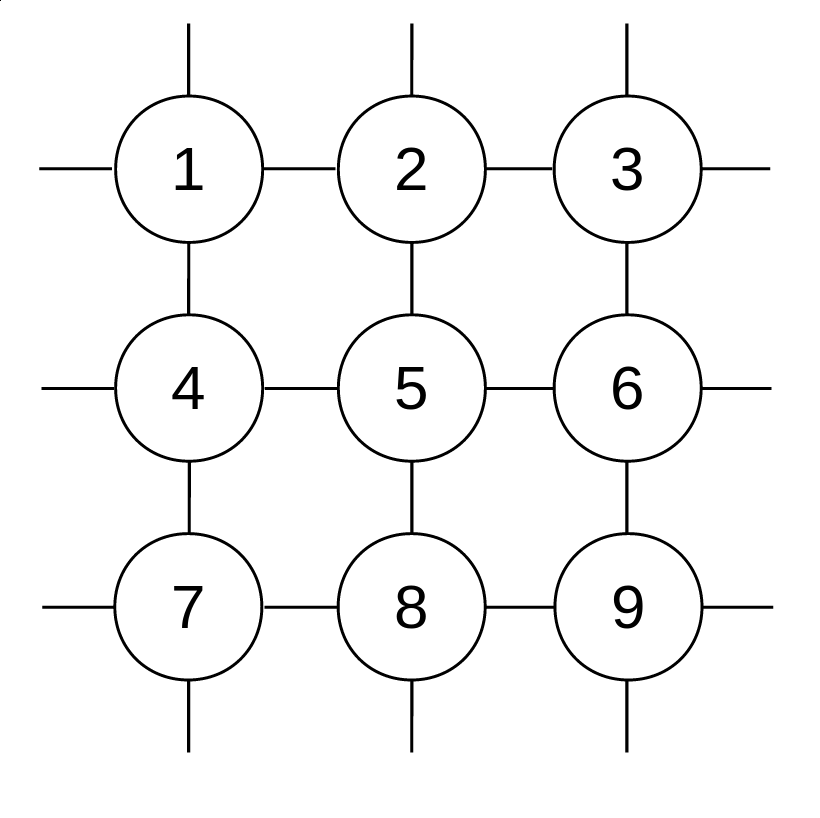
\includegraphics[width=0.9\linewidth]{figures/crowdsgrid.png}
\vspace{-4mm}
\caption{$3{\times}3$ instance of grid-Crowds.}
\label{figure:crowdsgrid}
\vspace{-6mm}
\end{wrapfigure}
Other than this limitation, the protocol works as the original: upon receiving a request, each user forwards to a user \review{with whom he can communicate} (including \review{himself}) with probability $p_f$, or sends it directly to the server with probability $1{-}p_f$. 
In this scenario, even if there are no corrupt users, the server can infer 
some information about the originator of the request. 
For example, if the server receives a request from user 2 in 
Figure~\ref{figure:crowdsgrid}, there is a greater chance that 
it was originated by user 1 than by user 6.

On this grid variation, the information leakage of the protocol depends 
not only on the number of corrupt users and on $p_f$, but also on where 
the corrupt users are located in the grid. 
\review{One of our goals is} to study the effects these topological variations have on 
QIF measures.